\section{Two scoring instruments}
\label{sec:instruments}

Phase~2 ran two auditor modes as separate campaigns.
Continuous configs (prefix T2c) set \texttt{miScoringMode} to continuous.
The headline \MI{}/\MPR{} is the continuous auditor float.
Dual configs (prefix T2d) call both a discrete auditor and a continuous sidecar on the same events.
The dual \emph{headline} is the discrete $0$--$5$ score.
The sidecar continuous value is a scoring diagnostic.
Dual gap (discrete minus sidecar continuous) is not a third ground-truth \MPR{}.

These two headlines are not the same quantity.
Dual-discrete H ($1.6814$) is not \enquote{the same \MPR{} as continuous H ($0.8643$) but higher}.
The auditors are different instruments.
Dual-discrete sits higher than continuous on every topology in this harvest.
That pattern is a scoring-mode effect.
It is not evidence that the discrete campaign found more misinformation in a shared unit.

\Cref{tab:headlines} reports live-cell means of \texttt{meanMI}.
Dead cells are excluded.
H and He remain separate.
The harvest cross-check on H matches the recomputed live means to four decimals.

\begin{table}[t]
\centering
\caption{Live-cell headline \MPR{} by arm and instrument.
Dead cells excluded.
$N=1$.
Do not pool the two columns or the two rows.}
\label{tab:headlines}
\begin{threeparttable}
\small
\begin{tabular}{lrrrr}
\toprule
Arm & Cont.\ \MPR{} (T2c) & $n$ live cont. & Dual-disc.\ \MPR{} (T2d) & $n$ live dual \\
\midrule
H (homogeneous) & 0.8643 & 480 & 1.6814 & 478 \\
He (heterogeneous) & 1.0192 & 238 & 2.0800 & 240 \\
\midrule
He $-$ H (same mode only) & 0.1549 & --- & 0.3986 & --- \\
Mean dual gap (sidecar) & --- & --- & 0.8804 (H) / 1.1145 (He) & --- \\
\bottomrule
\end{tabular}
\end{threeparttable}
\end{table}

The same cells as \texttt{meanNodeMPR} (not interchangeable with \texttt{meanMI}) are H continuous $0.8630$, H dual $1.6839$, He continuous $1.0140$, He dual $2.0737$.
This chapter leads with \texttt{meanMI} and treats \texttt{meanNodeMPR} as a sidecar of the same instrument.

\Cref{fig:dualgap} plots dual gap and agreement.
The gap is large on both arms.
Using it as an \MPR{} would smuggle the discrete--continuous disagreement into a third league table.
The figure is a diagnostic only.

\begin{figure}[t]
\centering
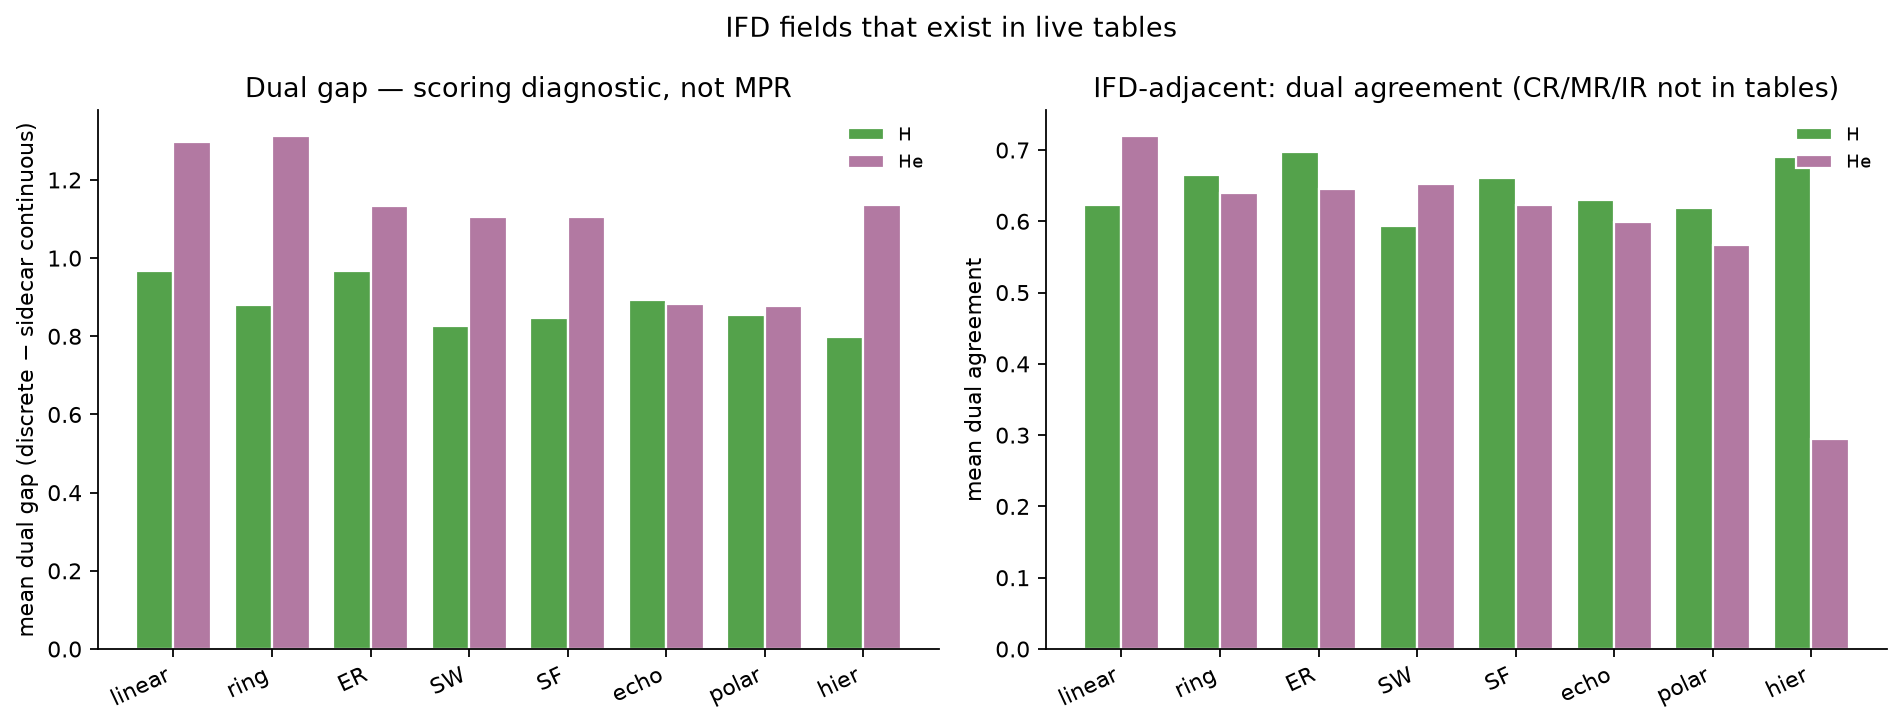
\includegraphics[width=\textwidth]{figures/fig20_ifd_dual_gap_agreement.png}
\caption[Dual gap and agreement]{Dual gap (discrete headline minus sidecar continuous) and dual agreement.
The gap is a scoring diagnostic, not a ground-truth \MPR{}.
$N=1$, eight hops.
Source: \texttt{fig20\_ifd\_dual\_gap\_agreement.png}.}
\label{fig:dualgap}
\end{figure}
